\chapter{Bayesian Model Inference \label{Chap:data:dcm_bms}}

This chapter describes the use of SPM's Bayesian Model Inference capabilities.
For a fuller background on this topic see \cite{dcm_families}.
We illustrate the methods using a DCM for fMRI study of the language system.

\section{Background}

The neuroimaging data derive from an fMRI study on the cortical dynamics of intelligible speech \cite{leff_speech}. 
This study applied dynamic causal modelling of fMRI responses to investigate  activity among three key multimodal regions: the left posterior and anterior superior temporal sulcus (subsequently referred to as regions P and A respectively) and pars orbitalis of the inferior frontal gyrus (region F). 
The aim of the study was to see how connections among regions depended on whether the auditory input was intelligible speech or time-reversed speech.

The basic DCM, from which all other models were derived, is shown in figure~\ref{dcms}. Auditory input enters region P and the three areas have full intrinsic connectivity. The modulatory input, encoding whether or not the auditory stimulus was speech or reversed speech, was then allowed to modulate a 
subset of connections in the model. These are the forward and backward connections between P and F, and the forward and backward connections between P and A. As these are either present or absent this results in $2^4=16$ different DCMs. 

\begin{figure}
\begin{center}
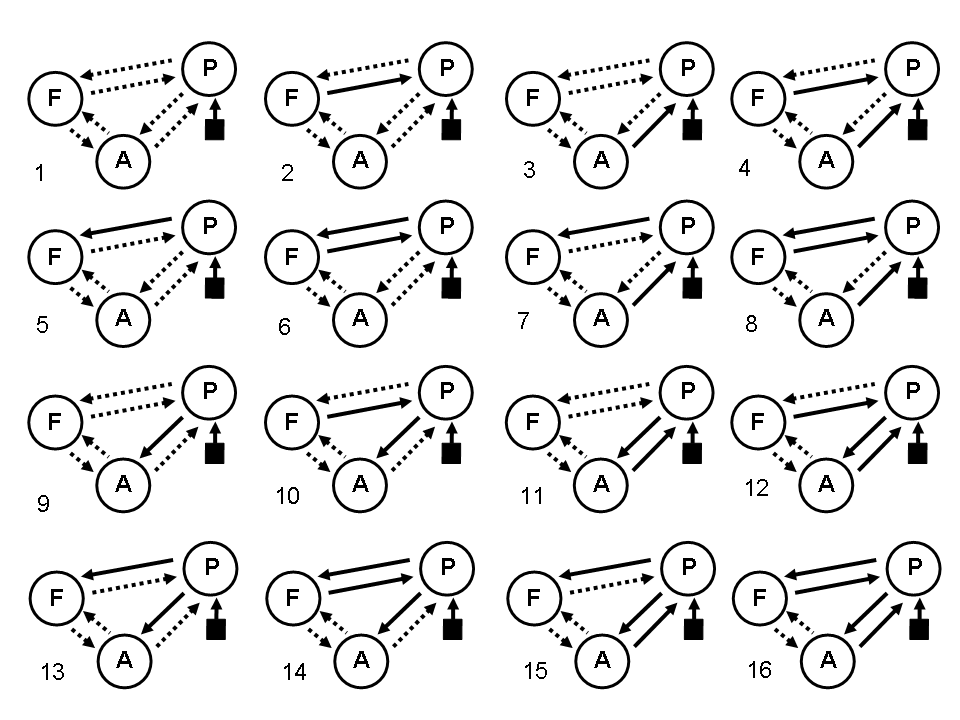
\includegraphics[width=100mm]{bms/Slide1.png}
\caption{All DCMs were fully connected ie. there were endogenous connections between all three regions (dotted lines) (i)  left posterior temporal sulcus (region P), (ii) left anterior superior temporal sulcus (region A) and (iii) pars orbitalis of the inferior frontal gyrus (region F). Auditory input enters region P. The sixteen models differ in their modulatory connectivity (solid lines) \label{dcms}}
\end{center}
\end{figure}

\section{Data}

An archive containing 16 DCMs for each of 12 subjects can be downloaded from the 
SPM web page\footnote{Bayesian comparison of Dynamic Causal Models: \url{http://www.fil.ion.ucl.ac.uk/spm/data/dcm_bms/}}. This archive is called \verb!dcm_bms.zip!. When you extract the data onto your computer a number of subdirectories will be created - one for each of the 12 subjects. The 16 DCMs for each subject are then available in these subject-specific directories. You can load one of these into SPM and examine the information contained therein. 

These DCM files contain the usual information eg. the original time series from each region of interest are available in
\verb!DCM.xY(1)! for region 1, wherein \verb!DCM.xY(1).name='PSTS_6'! indicates this is the posterior temporal region. The estimated parameter values are available in \verb!DCM.Ep!. You should note that these DCMs were specified and estimated using SPM revision 3894 (from May 2010) and that these DCM structures 
differ from earlier SPM releases.

Also in the Zip archive is a file called \verb!model_space.mat!. If you \verb!load model_space!, you will see that it contains a data structure called \verb!subj! with subfields 'sess' and then 'model'. If you type eg. \verb!subj(1).sess(1).model(1)! you will see four further subfields containing information about the first DCM for subject 1. This comprises the filename (fname), the free energy approximation to the model evidence (F), posterior mean parameters (Ep), and the posterior covariance of parameters (Cp).

The use of a `model space' file makes use of SPMs Bayesian model comparison (BMC) routines much simpler. If this file is not specified it will be automatically generated (from the DCM files) the first time you use the BMC routines (see below). Alternatively, you can easily create your own model space file. To get the current file to work on your system you will need to change all of the filenames (fname) so that they correspond to the positions of the DCM files in your filespace. You can do this with the \verb!model_space_filenames! function (also provided in the Zip archive).

\section{Analysis}

After unzipping the archive, correct the model space filenames using the 
command\newline \verb!subj=model_space_filenames(subj,new_base_dir)! where \verb!new_base_dir! is the name of the directory where you have unzipped the archive. This should be something like \newline \verb!'C:\blah\blah\blah\dcm-base-files'!. Then save \verb!subj! back in the model space file using \verb!save model_space subj!.

\subsection{Single Family}

Now open SPM and in the Menu window go to Batch, SPM, DCM, Bayesian Model Selection, Model Inference. This will open SPM's batch editor. Select an appropriate directory (eg. where you unzipped the archive), highlight Load model space and select the \verb!model_space.mat! file.
For inference method select 'FFX'. Save the batch job as \verb!ffx_all_models.mat!, then press the green play button to run the job.
This will produce the figure~\ref{ffx_model}, showing that model 6 is the best model.

\begin{figure}
\begin{center}
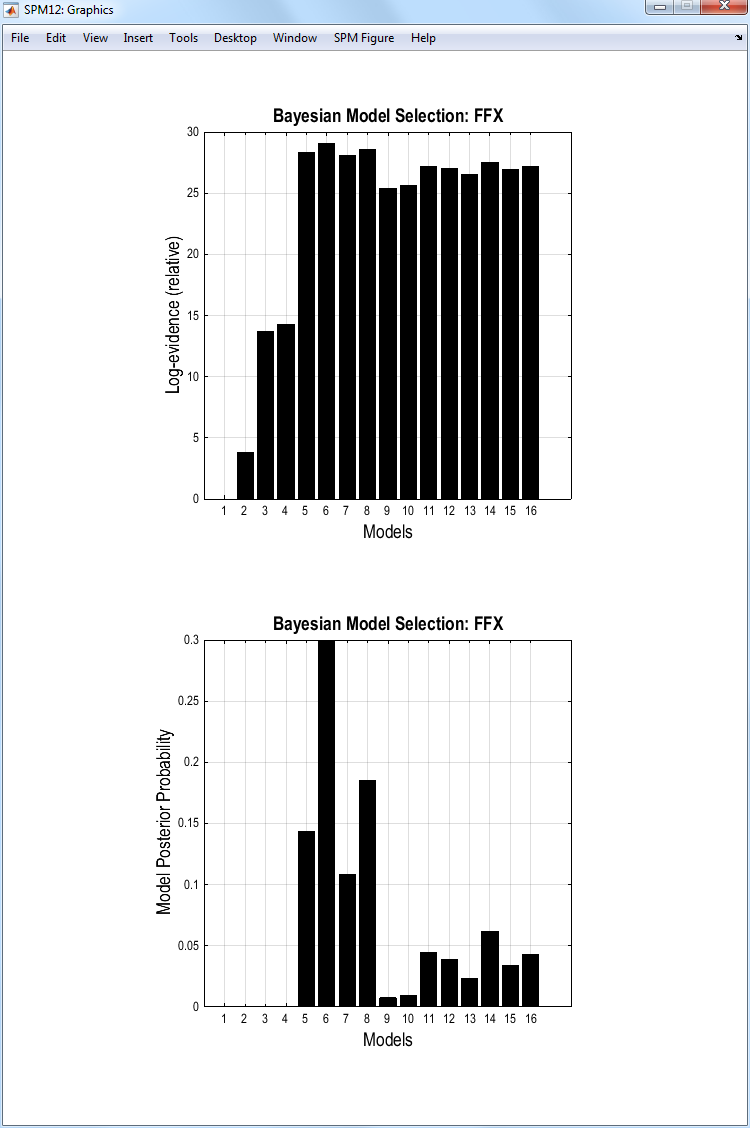
\includegraphics[width=150mm]{bms/Slide2.png}
\caption{Fixed effects model inference\label{ffx_model}}
\end{center}
\end{figure}

We can now go back and load the \verb!ffx_all_models.mat! job in the batch editor (press the Batch button) and change the inference methods to RFX. This will produce something like the results in figure~\ref{rfx_model} (note that the RFX approach uses a sampling procedure with a different random initial seed on each run, so the results can vary slighlty from run to run). Again, model 6 is the best model, but not by much. These RFX results will be stored in the same \verb!BMS.mat! file as the FFX results.

\begin{figure}
\begin{center}
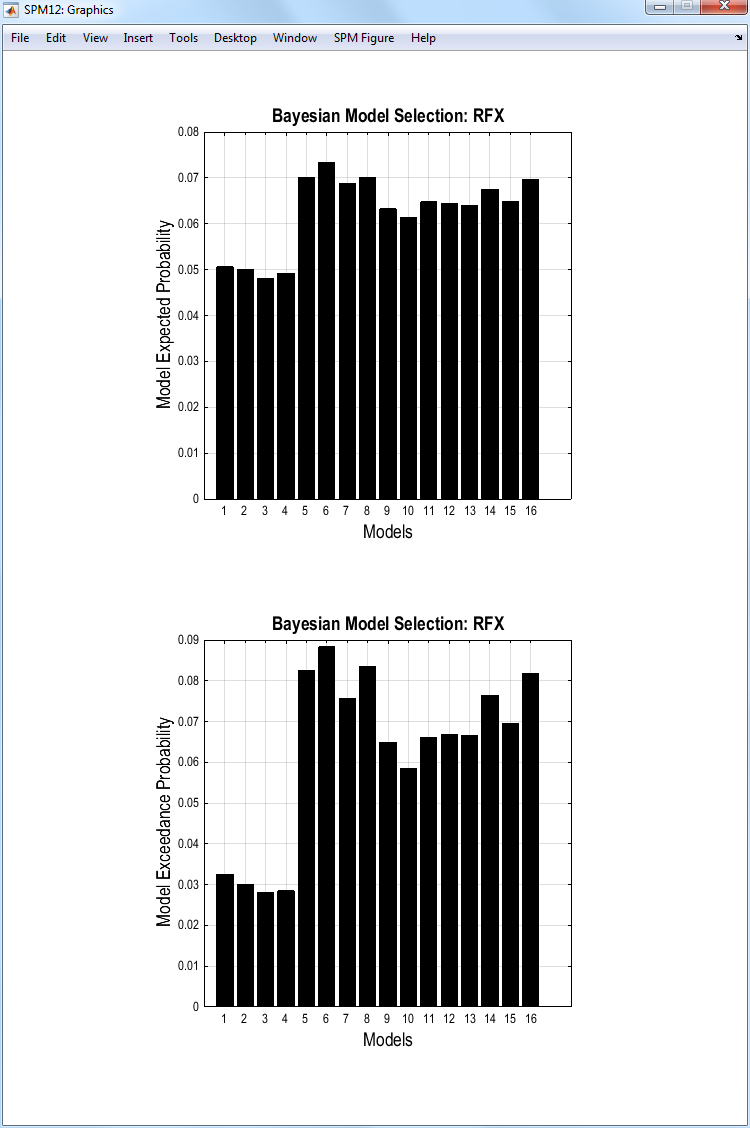
\includegraphics[width=150mm]{bms/Slide3.png}
\caption{Random effects model inference\label{rfx_model}}
\end{center}
\end{figure}

\subsection{Bayesian Model Averaging}

Now go back into the batch editor and reload the \verb!ffx_all_models.mat! job.
Highlight BMA, and select Choose family (instead of 'Do not compute'). Accept the 'Winning Family' option. The BMA results will be saved in the same BMS.mat file as the previous analyses. Now go ahead and press the green play button.
SPM will do the FFX model inference (again), but will also implement a weighted average of the model parameters where the weights are given by the evidence for each model, as described in \cite{dcm_families}. After the averaging is complete, SPM will report the number of models in Occams window. This should be 10 models (models 5,6,7,8,11,12,13,14,15,16). 

To look at the BMA results, go to the Menu window and press the Dynamic Causal Modelling button. Then select Average, select BMA, and then the BMS.mat file just created. If you then highlight the tab (top left) to select the modulatory variables you should get the plot shown in figure~\ref{bma}.

\begin{figure}
\begin{center}
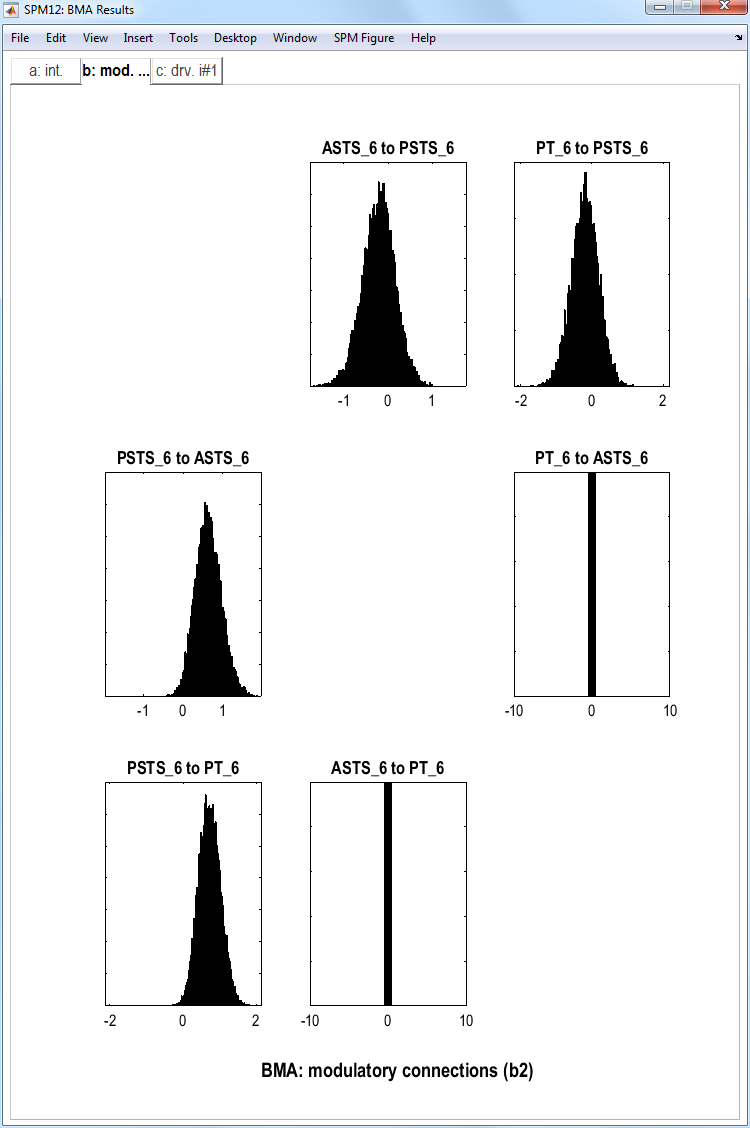
\includegraphics[width=150mm]{bms/Slide4.png}
\caption{Bayesian model averaging over all 16 models\label{bma}}
\end{center}
\end{figure}

\subsection{Family level inference}

The results so far have made no use of SPM's family inference procedure. 
Or rather, they have, but have assumed that all models belong to the same family. 

Open the \verb!ffx_all_models.mat! batch file again, highlight Family inference and select Load family. Highlight Load family and select the \verb!pf_family.mat! file contained in the Zip archive. This comprises two families (i) those with a forward connection from P to F ('PF'), and (ii) those without it ('No PF'). Set the BMA option to Do not Compute. Select a new directory you have created for this analysis (eg pf-family) and run the job.
SPM will create the family level inference plot shown in figure~\ref{family}.
This gives a 90\% posterior probability to models with the P to F connection.

We will now repeat the analysis but with RFX inference. You should see a result similar to that shown in
figure~\ref{rfx_family}.

\subsection{Summary Statistics and Group Analyses}

The group mean DCM parameters can be easily obtained from the \matlab\ command window by loading the \verb!BMS.mat! file and then typing: \verb!BMS.DCM.ffx.bma.Ep!.

The subject specific mean DCM parameters can be obtained as follows: \verb!BMS.DCM.ffx.bma.Eps(n)!, where $n$ is the subject number. For random-effects change \verb!ffx! to \verb!rfx!. 

If we are interested in the modulatory connection from region 1 to region 3 (that is modulated by the second input), then the mean value of this for Subject 10 is given by\newline \verb!BMS.DCM.ffx.bma.Eps(10).B(3,1,2)! (which should be 0.7475). The mean connection values for all subjects (12) can be gotten with the \matlab\ syntax \newline \verb!for i=1:12, b(i) = BMS.DCM.ffx.bma.Eps(i).B(3,1,2); end!.

These subject specific mean parameters can then act as summary statistics for a standard group analysis. For example to look for significant differences between eg. a control group and a patient group in a modulatory parameter one would implement a two-sample t-test on data from the appropriate entries in the \verb!mean_bs! matrices. Similarly, if one has 3 groups one would use a 3-level ANOVA.

\begin{figure}
\begin{center}
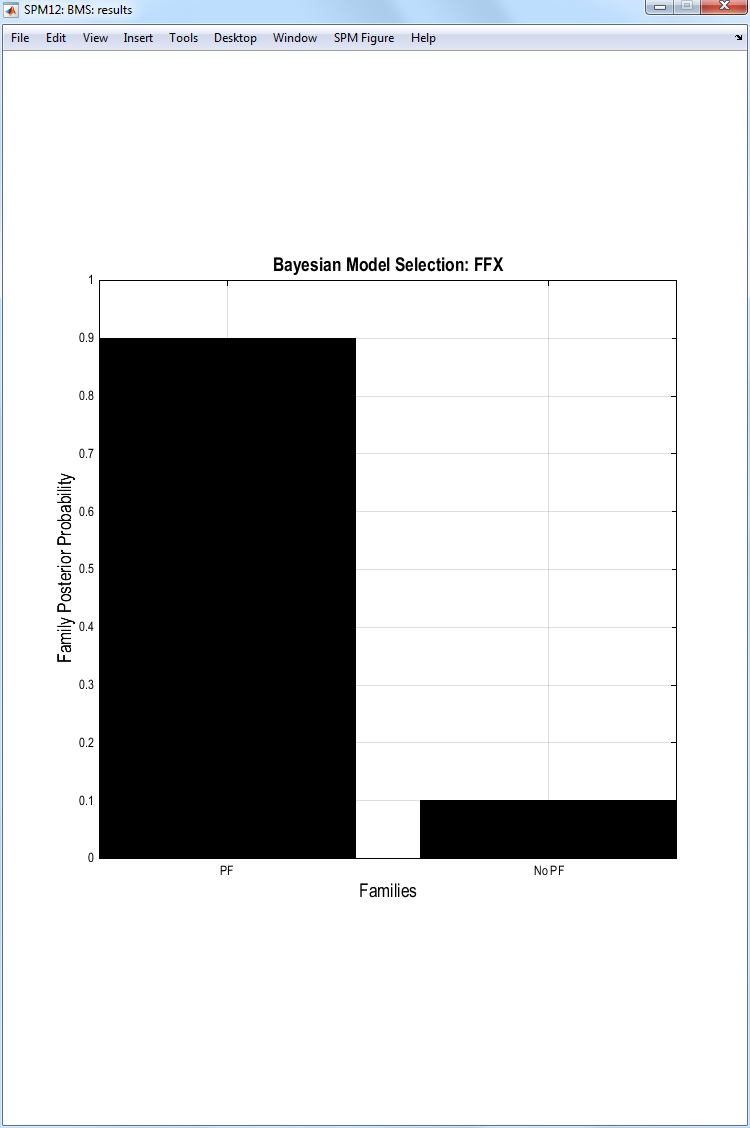
\includegraphics[width=150mm]{bms/Slide5.png}
\caption{FFX family inference\label{family}}
\end{center}
\end{figure}

\begin{figure}
\begin{center}
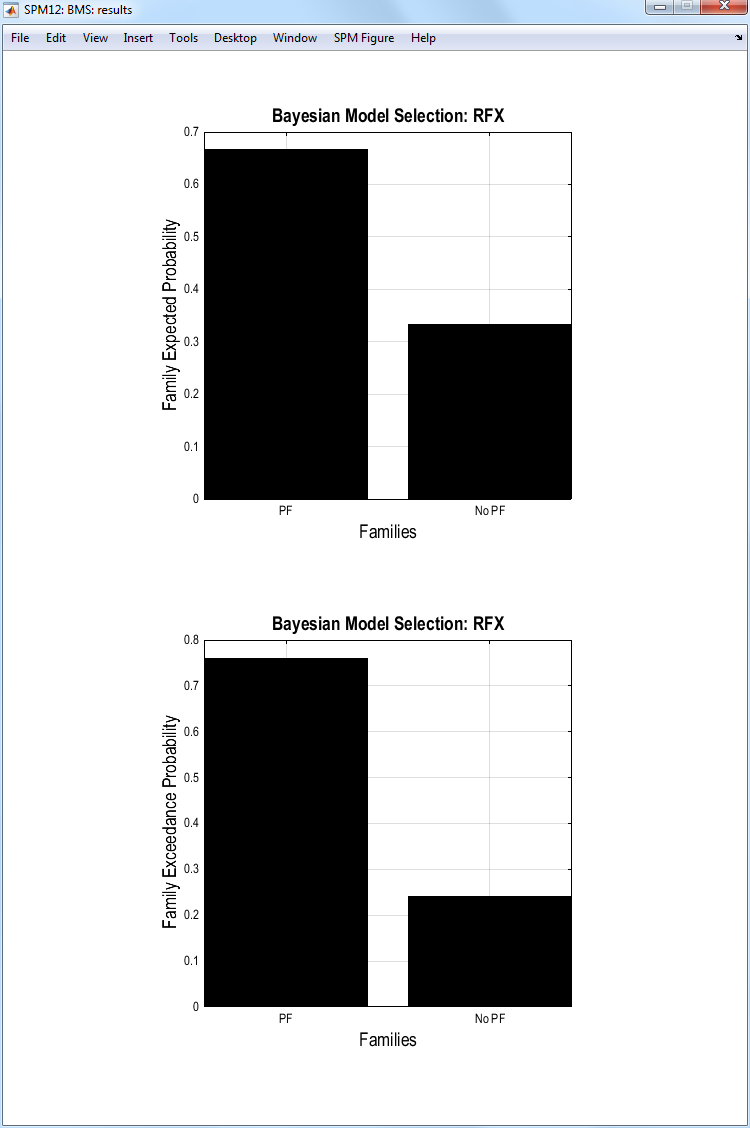
\includegraphics[width=150mm]{bms/Slide6.png}
\caption{RFX family inference\label{rfx_family}}
\end{center}
\end{figure}

\section{BMS.mat file}

The BMS structure saved in BMS.mat file contains the following variables\footnote{nm = number of models; nfam = number of families; nsub = number of subjects; nsamp = number of samples; dima/b/c/d = dimensions of a/b/c/d DCM parameters; np = number of model parameters; nsess = number of sessions.}:

\paragraph{BMS.DCM.ffx/rfx} (fixed-effects (FFX) / random-effects (RFX) analysis)\\\\

\begin{tabular}{ l l }
\bf{.data}          & path to model\_space.mat file (see below).  \\
\bf{.F\_fname} & path to file containing the log evidence matrix, F, (if this option is specified). \\
\bf{.F}                & matrix of log model evidences for all subjects and models, [nsub $\times$ nm].  \\
\bf{.SF} 	       & vector of summed log evidences over subjects [1 $\times$ nm]. \\
\bf{.model}       & results from model level inference (see below). \\
\bf{.family}       & results from family level inference (see below). \\
\bf{.bma}          & results from Bayesian model averaging (see below). \\
\end{tabular}

\subsection{Model level results}

\hspace{4mm} Fixed-effects:\\

\begin{tabular}{ l l l }
\bf{model}           & & \\
& \bf{.prior}          & model priors, $p(m)$, [1 $\times$ nm]. \\
& \bf{.subj\_lme} & log model evidence matrix, [nsub $\times$ nm]. \\
& \bf{.like}            & model likelihoods, $p(Y|m)$, [1 $\times$ nm]. \\
& \bf{.posts}        & model posterior probabilities, $p(m|Y)$, [1 $\times$ nm]. \\
\end{tabular}\\\\

Random-effects (different from fixed-effects):\\

\begin{tabular}{ l l l }
\bf{model}        & & \\
& \bf{.alpha0}  & initial Dirichlet parameters (prior counts), $\alpha_0$, [1 $\times$ nm].\\
& \bf{.exp\_r}   &  model posterior means, $<r|Y>$, [1 $\times$ nm].\\
& \bf{.xp}           & model exceedance probabilities, $\psi_m$ [1 $\times$ nm].\\
& \bf{.r\_samp} &  samples from the model posterior density, $p(r|Y)$, [nsamp $\times$ nm].\\
& \bf{.g\_post}  &  posterior model probabilities for subject n and model m, $p(m_n|Y)$, [nsub $\times$ nm].
\end{tabular}\\

\subsection{Family level results}

\hspace{4mm} Fixed-effects:\\

\begin{tabular}{ l l l }
\bf{family}         & & \\
& \bf{.names}   & family names, ex: $\{$`F1', `F2', `F3'$\}$.\\
& \bf{.partition} & partition vector assigning each model to a family [1 $\times$ nm].\\
& \bf{.infer	}       & inference method (`ffx' or `rfx').\\
& \bf{.prior}       & family priors, $p(f_k)$, [1 $\times$ nfam].\\
& \bf{.post}       & family posterior probabilities, $p(f_k|Y)$, [1 $\times$ nfam].\\
& \bf{.like}        & family likelihoods, $p(Y| f_k)$, [1 $\times$ nfam].
\end{tabular}\\\\

Random-effects (different from fixed-effects):\\

\begin{tabular}{ l l l }
\bf{family}         & & \\
& \bf{.Nsamp}  & number of samples used in Gibbs� sampling (default = 20000).\\
& \bf{.prior	}        & family type of priors (`F-unity', $\alpha_0=1$, for each family, is the default; \\
& & other option, `M-unity',  $\alpha_0=1$, for each model) .\\
& \bf{.alpha0}    & initial values of the Dirichlet parameters (prior counts), $\alpha_{prior}(m)$, [1 $\times$ nfam].\\
& \bf{.s\_samp}  & samples from family posterior density, $p(s|Y)$, [nsamp $\times$ nfam].\\
& \bf{.exp\_r}      & family posterior means, $<s_k|Y>$, [1 $\times$ nfam].\\
& \bf{.xp}	          & family exceedance probabilities, $\psi_k$, [1 $\times$ nfam].
\end{tabular}\\

\subsection{Bayesian model averaging (BMA)}

\hspace{4mm} Fixed-effects:\\

\begin{tabular}{ l l l }
\bf{bma} & & \\
& \bf{.nsamp} &	 number of samples used to average parameters (default = 10000). \\
& \bf{.oddsr} & posterior odds ratio, $\pi_{OCC}$, (number of models in Occam�s window, \\
& & default = 0). \\
& \bf{.Nocc} & number of models in Occam's window. \\
& \bf{.Mocc} & index of models in Occam's window, [1 $\times$ nm]. \\  
& \bf{.indx} & index of models in Occam's window (different for each subject in RFX),\\
& &  [1 $\times$ nm]. \\
& \bf{.a} & samples from posterior density over DCM.a parameters [dima $\times$ nsamp]. \\
& \bf{.b} & samples from posterior density over DCM.b parameters [dimb $\times$ nsamp]. \\
& \bf{.c} & samples from posterior density over DCM.c parameters [dimc $\times$ nsamp]. \\
& \bf{.d} & samples from posterior density over DCM.d parameters [dimd $\times$ nsamp]. \\
& \bf{.mEp} & mean DCM parameters [1 $\times$ 1 struct]. \\
& \bf{.sEp} & standard deviation of DCM parameters [1 $\times$ 1 struct]. \\
& \bf{.mEps} & mean DCM parameters per subject [1 $\times$ nsub struct]. \\
& \bf{.sEps} & standard deviation DCM parameters per subject [1 $\times$ nsub struct]. \\
\end{tabular}\\\\

Random-effects - same variables as in fixed-effects.

\section{model\_space.mat file}

This structure is created automatically if it doesn't exist in the chosen directory and can be loaded for subsequent analyses as a faster option to reading the DCM.mat files. The model\_space.mat file contains the following structure:\\\\

\begin{tabular}{ l l l }
\bf{subj(nsub).sess(nsess).model(nm)} & & \\
 & \bf{.fname} 	& path to DCM.mat file. \\
 & \bf{.F}		& log-evidence (free energy). \\ 
  & \bf{.Ep}		& parameter estimates: conditional expectation,\\
  & &  [np $\times$ 1]. \\
& \bf{.Cp}		& parameter estimates: conditional covariance,\\
& &  [np $\times$ np]. 
\end{tabular}\\\\

For a detailed description of all the variables and methods please see \cite{dcm_families} and \cite{klaas_bms}.

